
%------------------------ Start chapter 3 -------------
\cchapter{روش حل مسئله}
\pagebreak

\section{مقدمه}
 این پروژه در دو بخش کلی پیش‌پردازش در سمت سخت‌افزار و پردازش در سرور انجام شده‌است. در بخش اول، تعدادی پردازش اولیه بر روی داده‌های خام ضربان قلب انجام می‌شود. این بخش یک بستر پیاده شده بر روی سخت‌افزار است که برای کامل شدن باید به یک سنسور ضربان قلب متصل شود. این بخش همراه بیمار خواهد بود و پردازش‌های ساده‌ی اولیه را بر روی سیگنال نوار قلب انجام داده و نتایج را به سرور ارسال می‌کند.  پردازش‌های پیچیده‌تر برای تشخیص آریتمی بر عهده‌ی سرور خواهد بود. در سرور یک الگوریتم دسته‌بندی بر روی داده‌ها انجام شده و کلاس آریتمی آن‌ها تشخیص داده می‌شود.

\section{عملیات پیش‌پردازش بر روی سخت‌افزار} 
در این بخش عملیات پیش‌پردازش با هدف تشخیص ترکیب \lr{QRS} در هر ضربان قلب بر روی سیگنال دیجیتال ضربان قلب اجرا می‌شود. خروجی این عملیات، موقعیت زمانی قله‌ی \lr{R} در ترکیب \lr{QRS} هر ضربان است که در پردازش‌های آینده برای تشخیص آریتمی آن ضربان مورد استفاده قرار می‌گیرد. این بخش بر روی یک ماژول \lr{ESP8266} که یک ماژول وای‌فای دارای یک پردازنده‌ی ۸۰ مگاهرتزی است، پیاده‌سازی می‌شود. این ماژول علاوه بر انجام پیش‌پردازش، ارسال داده‌‌های حاصل از آن از طریق وای‌فای را نیز بر عهده دارد. قسمت‌های پیاده‌سازی‌شده در این بخش در شکل \ref{fig:preprocessing} در کادر مشخص شده‌اند.
\begin{figure}[!htb]
\centering
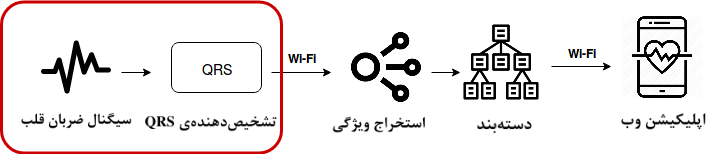
\includegraphics[width=16cm]{Figures/preprocessing.png}
\caption{بخش پیش‌پردازش بر روی سخت‌افزار در مراحل تشخیص آریتمی}
\label{fig:preprocessing}
\end{figure}
	\subsection{مراحل تشخیص QRS}

	پیش از ورود سیگنال نوار قلب به ماژول پیش‌پردازش، نوار قلب خام گرفته‌شده از بیمار  از یک مبدل آنالوگ به دیجیتال\LTRfootnote{ADC} عبور کرده و با نرخ نمونه‌برداری\LTRfootnote{Sampling rate} معینی به سیگنال دیجیتال تبدیل می‌شود. مقدار این نرخ نمونه‌برداری در برخی مراحل پیش‌پردازش اهمیت دارد. 
پس از دیجیتال شدن، سیگنال وارد ماژولی که برای تشخیص \lr{QRS} طراحی کرده‌ایم می‌شود. در ادامه به مراحل اصلی طی‌شده در این بخش می‌پردازیم.
		\subsubsection{حذف نویز سیگنال به کمک فیلتر میان‌گذر}
		اولین مرحله در تشخیص \lr{QRS} حذف نویز سیگنال نوار قلب است. در حین ثبت ضربان قلب، منابع مختلفی از نویز در سیگنال اختلال ایجاد می‌کنند. در یک سیگنال ECG به طور معمول نویزهای فرکانس پایینی ناشی از نوسانات الکترود مرجع وجود دارد. این نویزها به علت حرکت الکترودها بر روی پوست و همین طور اعمالی چون حرکات و تنفس بیمار به وجود می‌آیند. انقباض ماهیچه‌های اطراف قلب نیز یکی دیگر از منابع نویز است. این انقباضات توسط الکترودها ثبت شده و در نوار قلب نویزهای فرکانس بالایی ایجاد می‌کنند.\cite{Joshi2013}
		
		با توجه به نویزهای معمول، محدوده‌ی فرکانسی مطلوب برای بیشینه‌کردن انرژی QRS و کمینه‌کردن انرژی نویز، ۵ تا ۱۵ هرتز تشخیص داده شده‌است.\cite{Pan1985} به منظور نگه‌داشتن این بازه‌ی فرکانسی و حذف فرکانس‌های بالا و پایین آن، سیگنال دیجیتال از یک فیلتر میان‌گذر عبور داده می‌شود. این فیلتر متشکل از یک فیلتر پایین‌گذر و یک فیلتر بالاگذر متوالی است. هر دوی این فیلترها به صورت نرم‌افزاری پیاده‌سازی شده‌اند.
تابع تبدیل فیلتر پایین‌گذر را در معادله‌ی \ref{eq:lowpassTr} مشاهده می‌کنیم.

\begin{equation}
	H(z) = \frac{{(1-z^{-6})}^2}{{(1-z^{-1})}^2}
\label{eq:lowpassTr}
\end{equation}
	
	معادله‌ی تفاضلی این فیلتر به صورت معادله‌ی \ref{eq:lowpassDE} در خواهد آمد.
	
\begin{equation}
	y(nT) = 2y(nT-T) - y(nT-2T) + x(nT) - 2x(nT-6T) + x(nT-12T) 
\label{eq:lowpassDE}
\end{equation}
فرکانس قطع این فیلتر پایین‌گذر ۱۱ هرتز و بهره‌ی آن ۳۶ است. یک فیلتر بالاگذر به صورت سری با این فیلتر قرار می‌گیرد که تابع تبدیل آن به صورت معادله‌ی \ref{eq:highpassTr} است.
\begin{equation}
	H(z) = \frac{{(-1+32z^{-16}+z^{-32})}}{{(1+z^{-1})}}
\label{eq:highpassTr}
\end{equation}
که معادله‌ی تفاضلی آن به صورت معادله‌ی \ref{eq:highpassDE} خواهد بود.
 \begin{equation}
	y(nT) = 32x(nT-16T) - [y(nT-T) + x(nT) - x(nT-32T)]
\label{eq:highpassDE}
\end{equation}
این فیلتر فرکانس‌های بالای ۵ هرتز را عبور می‌دهد و بهره‌ی آن ۳۲ است. از توالی این دو فیلتر، فیلتر میان‌گذری به دست می‌آید که فرکانس‌های ۵ تا۱۱ هرتز را عبور می‌دهد که به هدف ما برای کاهش نویز نزدیک است. 

\subsubsection{مشتق‌گیر}
پس از اعمال فیلترها، عمل مشتق‌گیری بر روی سیگنال انجام می‌شود. مشتق‌گیری از سیگنال، اطلاعاتی در مورد شیب آن در بازه‌ی QRS فراهم می‌کند. تابع انتقال این فیلتر به صورت معادله‌ی \ref{eq:derivativeTr} است و معادله‌ی تفاضلی آن به صورت رابطه‌ی \ref{eq:derivativeDE} می‌آید.

\begin{equation}
	H(z) = \frac{(-z^{-2}-2z^{-1}+2z+z^2)}{8T}
\label{eq:derivativeTr}
\end{equation}
	
\begin{equation}
	y(nT) = \frac{-x(nT-2T)-2x(nT-T)+2x(nT+T)+x(nT+2T)}{8T}
\label{eq:derivativeDE}
\end{equation}

\subsubsection{مجذورکننده}
پس از مشتق‌گیری، مجذور سیگنال به صورت نقطه به نقطه به دست می‌آید. معادله‌ی تفاضلی فیلتر در این بخش به صورت معادله‌ی \ref{eq:square} است. اعمال این فیلتر بر روی خروجی مشتق‌گیر، باعث می‌شود تمامی نقاط سیگنال مثبت شده و به دلیل انجام عمل مربع‌کردن، فواصل نقاط گسسته‌ی سیگنال تشدید شود.

\begin{equation}
	y(nT) = [x(nT)]^2
\label{eq:square}
\end{equation}

\subsubsection{انتگرال‌گیر با پنجره‌ی لغزان}
در این مرحله سیگنال مربع‌شده وارد یک انتگرال‌گیر می‌شود. هدف از این کار، به دست آوردن اطلاعاتی در مورد شکل موج سیگنال، علاوه بر اطلاعات مربوط به شیب موج R است که در مراحل قبل به دست آمد. معادله‌ی تفاضلی این انتگرال‌گیر به صورت معادله‌ی \ref{eq:integrator} است.

\begin{equation}
	y(nT) = \frac{x(nT-(N-1)T) + x(nT-(N-2)T+...+x(nT))}{N}
\label{eq:integrator}
\end{equation}

که در آن N تعداد نمونه‌ها در طول پنجره‌ی انتگرال‌گیر است. $N$ به صورت تجربی به دست می‌آید و در تشخیص نهایی \lr{R} اهمیت زیادی دارد. به طور معمول $N$ باید تقریبا به اندازه‌ی عریض‌ترین بازه‌ی \lr{QRS} باشد. در صورتی که پنجره بیش از حد عریض باشد، در هنگام انتگرال‌گیری، شکل موج \lr{QRS} با موج \lr{T} ترکیب می‌شود. اگر پنجره بیش از حد کوتاه باشد، کل بازه‌ی \lr{QRS} را در بر نمی‌گیرد و در این بازه تعداد زیادی قله تولید خواهد شد. این مقدار به طور تجربی به دست آمده و با نرخ نمونه‌برداری ارتباط دارد. در این پروژه طول پنجره ۷۰ در نظر گرفته شده‌است.

\subsubsection{تعیین موقعیت قله‌های R با کمک مقدارهای آستانه}

موج \lr{QRS} هم‌زمان با لبه‌ی بالارونده‌ی انتگرال‌گیر رخ می‌دهد، و طول بازه‌ی این لبه برابر با طول بازه‌ی \lr{QRS} است. به این ترتیب، می‌توان موقعیت زمانی \lr{QRS} را از روی جایگاه لبه‌ی بالارونده تعیین کرد. با استفاده از این اطلاعات، و همین طور اطلاعات مربوط به شیب منحنی \lr{QRS} در این بازه، می‌توان نقطه‌ی ثابتی را به عنوان موقعیت قله‌ی \lr{R} به دست آورد.
برای تعیین درست موقعیت قله‌ی \lr{R} تعدادی ولتاژ آستانه\LTRfootnote{Threshold}اعمال می‌شوند و به نسبت بالاتر یا پایین‌تر بودن ولتاژ هر نمونه از آن‌ها، وجود یا عدم وجود قله تشخیص داده می‌شود. این آستانه‌ها با گذشت زمان با نویز تطبیق می‌یابند. در مجموع دو سری ولتاژ آستانه داریم که هر کدام شامل دو آستانه هستند. در هر یک از این دو سری، آستانه‌ی بالاتر برای تحلیل اولیه‌ی سیگنال استفاده می‌شود، و در صورتی که در یک بازه‌ی زمانی مشخص \lr{QRS} ای تشخیص داده نشده باشد، لازم است در این بازه از تکنیک جستجوی برگشتی\LTRfootnote{Search-back} استفاده شود. در این تکنیک در این بازه‌ی زمانی  از آستانه‌های پایین‌تر برای تشخیص \lr{QRS} استفاده می‌شود. روابط این آستانه‌ها در معادله‌ی \ref{eq:thresholds} مشاهده می‌شوند. در این روابط، \lr{PEAK1} بالاترین ولتاژ سیگنال به طور کلی، \lr{SPKI} تخمین جاری از بالاترین ولتاژ سیگنال و \lr{NPKI} تخمین جاری از بالاترین ولتاژ نویز در هر لحظه است. همچنین  \lr{TH I1} اولین مقدار آستانه‌ی اعمال‌شده بر روی سیگنال انتگرال‌گیری‌شده و \lr{TH I2} دومین مقدار آستانه و نصف مقدار آستانه‌ی اول است.

\begin{align}
\begin{split}
	& SPKI = 0.125 PEAKI + 0.875 SPKI\\
	& NPKI = 0.125 PEAKI + 0.875 NPKI\\
	& TH\: I1 = NPKI + 0.25(SPKI - NPKI)\\
	& TH\:I2 = 0.5 TH I1\\
\end{split}
\label{eq:thresholds}
\end{align}
برای این که یک نمونه به عنوان قله‌ی \lr{R} تشخیص داده شود، باید مقداری بالاتر از \lr{TH I1} داشته باشد. در صورتی که یک قله‌ی \lr{R} در فرایند جستجوی برگشتی تشخیص داده شود، مقدار \lr{SPKI} به صورت رابطه‌ی \ref{eq:thresholdSPKI} به‌روز خواهد شد. 
\begin{equation}
	SPKI = 0.25 PEAKI + 0.75 SPKI
\label{eq:thresholdSPKI}
\end{equation}

	\subsection{پیاده‌سازی الگوریتم تشخیص QRS بر روی بستر سخت‌افزاری}
	
ورودی این بخش، سیگنال دیجیتال دریافت شده از سنسور ضربان قلب است. نحوه‌ی تولید این سیگنال و نوع سنسور به‌کاررفته برای آن کاملا به کاربرد بستگی داشته و در این پروژه تاکیدی بر روی آن نیست. محاسبات انجام‌شده در الگوریتم تشخیص \lr{QRS}، به مقدار نرخ نمونه‌برداری سیگنال ضربان قلب وابسته است. پارامترهای الگوریتم پیاده‌سازی شده در این بخش، برای نرخ نمونه‌برداری ۳۶۰ نمونه بر ثانیه بهینه شده‌اند و از این روی، لازم است نرخ نمونه‌برداری سیگنال دیجیتال ورودی، مساوی با ۳۶۰ یا نزدیک به آن باشد.

خروجی این بخش، موقعیت زمانی قله‌ی \lr{R} در هر یک از بازه‌های \lr{QRS} تشخیص‌داده‌شده در ضربان قلب است. به بیان دیگر، الگوریتم برخی از نمونه‌ها در سیگنال را به عنوان قله‌ی \lr{R} تشخیص داده و شماره‌ی آن نمونه را به عنوان خروجی برمی‌گرداند. این مقادیر باید برای انجام پردازش‌های آینده به سرور ارسال شوند. از آن‌جا که از کل سیستم انتظار بی‌درنگ‌بودن داریم، علاوه بر تشخیص بی‌درنگ \lr{QRS} لازم است دریافت داد‌ه‌های خام از حسگر و همین‌طور فرستادن قله‌های \lr{R} تشخیص‌داده‌شده به سرور نیز به صورت بی‌درنگ و در حین تشخیص \lr{QRS} انجام شود. به بیان بهتر، در چنین کاربردی انجام تشخیص \lr{QRS} بر روی ضربان قلب به طور کامل و سپس فرستادن تمامی \lr{R}های تشخیص‌داده‌شده به سرور قابل قبول نخواهد بود.
کارهای انجام‌شده در این بخش را می‌توان در قالب موارد زیر بیان کرد. 
\subsubsection{دریافت داده‌های خام جدید از حس‌گر}
در این بخش، هدف بر این است که رفتار یک حس‌گر دیجیتال ضربان قلب با نرخ نمونه‌برداری ۳۶۰ نمونه بر ثانیه شبیه‌سازی شود. بهترین راه‌حل برای این کار، استفاده از ارتباط سریال بین ماژول و یک رایانه (به جای حس‌گر) تشخیص داده شد. با فرض این که داده‌های چنین حس‌گری قبلا دریافت و بر روی رایانه ذخیره شده باشد، در صورتی که در هر ثانیه ۳۶۰ نمونه از رایانه به ESP ارسال کنیم، رفتار یک حس‌گر دیجیتال با نرخ نمونه‌برداری ۳۶۰ را شبیه‌سازی کرده‌ایم.

پیاده‌سازی این بخش به این صورت انجام شد که پایه‌های \lr{RX} و \lr{TX} ماژول \lr{ESP8266} به پورت سریال یک کامپیوتر وصل شد و داده‌های دیجیتال ضربان قلب که قبلا به وسیله‌ی یک حس‌گر دیجیتال تولید شده بودند،‌ به وسیله‌ی اسکریپتی در کامپیوتر به \lr{ESP8266} ارسال شدند. در هر ثانیه ۳۶۰ مقدار از مقادیر ذخیره شده با نرخ باد ۱۱۲۵۰۰ بیت بر ثانیه به \lr{ESP8266} ارسال شدند. \lr{ESP8266} این داده‌ها دریافت کرده و پردازش‌های آینده را بر روی آن‌ها انجام خواهد داد. این ماژول به طور دائم در حال اجرای الگوریتم تشخیص \lr{QRS} بر روی داده‌هایی که قبلا دریافت کرده است می‌باشد، و در این حین داده‌های جدیدی نیز از سمت رایانه (حس‌گر) دریافت می‌کند.
\subsubsection{اعمال الگوریتم و فرستادن شماره‌ی نمونه به  سرور
 در صورت تشخیص قله}
	 هدف این بخش این است که  ماژول \lr{ESP8266} الگوریتم تشخیص \lr{QRS} را بر روی نمونه‌هایی که دریافت می‌کند اجرا کرده و در صورت تشخیص قله، موقعیت زمانی آن را برای سرور بفرستد. در همین حین، هر لحظه نمونه‌های جدیدی از طریق ارتباط سریال دریافت می‌شوند. چالش به‌وجودآمده در این مرحله این است که این نمونه‌های جدید نباید از دست بروند. یک راه حل ممکن برای این موضوع،‌ پیاده‌سازی نوعی مکانیزم چندنخی\LTRfootnote{Multithreading} در \lr{ESP8266} است. در یکی از نخ‌ها، داده‌های جدید دریافت شوند و در نخ دیگر الگوریتم بر روی داده‌‌های موجود اجرا شود.
	 
با بررسی‌های انجام‌شده دریافت شد که پیاده‌سازی چندنخی بر روی \lr{ESP8266} پیچیدگی بالایی داشته و کارا نمی‌باشد. به جای پیاده‌سازی این روش، از امکان ایجاد وقفه‌ی سریال در هنگام دریافت داده استفاده شد. \lr{ESP8266} امکان دریافت داده‌ها به صورت مبتنی بر وقفه را دارد، که در کتاب‌خانه‌ی \lr{HardwareSerial} به طور کامل پیاده‌سازی شده است. نحوه‌ی پیاده‌سازی به این شکل است که به محض ورود داده‌ی سریال جدید، \lr{ESP8266} کار خود را رها کرده و به وقفه سرویس می‌دهد. در روتین وقفه، کاراکتر تازه وارد از طریق ارتباط سریال، در بافر سریال \lr{ESP8266} می‌شود. سپس برنامه از روتین وقفه خارج شده و به ادامه‌ی کار خود باز می‌گردد. با استفاده از این امکان \lr{ESP8266} قادر است به طور همزمان با اجرای الگوریتم، نمونه‌های جدید را دریافت کند.

 به دلیل محدود بودن حجم بافر سریال داخلی موجود در \lr{ESP8266}، نیاز به پیاده‌سازی یک مکانیزم بافرینگ در خود کد نیز وجود دارد. برای جلوگیری از سرریز کردن بافر سریال، در ابتدای هر لوپ اجرای برنامه‌ی \lr{ESP8266} به این بافر سرکشی شده و داده‌های جدید را از آن بر می‌داریم و در بافری که خود پیاده‌سازی کرده‌ایم قرار می‌دهیم. این بافر برای اطمینان حجم بیشتری دارد و با استفاده از آرایه پیاده‌سازی شده‌است. داده‌های جدید در این آرایه می‌مانند، تا وقتی که نوبت پردازش و انجام الگوریتم روی آن‌ها فرا برسد.

	

\section{عملیات پردازش سمت سرور}
بخش دوم سیستم با استفاده از الگوریتم‌های یادگیری ماشین، و بر روی یک سرور پیاده‌سازی شده‌است. نتایج پیش‌پردازش‌های انجام شده در بخش قبل در سرور دریافت شده و ویژگی‌های هر ضربان استخراج می‌شود. سپس با استفاده از این ویژگی‌ها، عمل دسته‌بندی ضربان‌ها انجام شده و به هر ضربان یک برچسب که تعیین‌کننده‌ی کلاس ضربان است، اختصاص داده می‌شود. در شکل \ref{fig:server} مراحل پیاده‌سازی‌شده در این بخش در کادر مشخص شده‌اند. سرور مشخص‌شده در این تصویر، یک دامنه است که کاربران می‌توانند با واردکردن آدرس آن در مرورگرهای خود، از هر کجا به آن متصل شوند.

\begin{figure}[!htb]
\centering
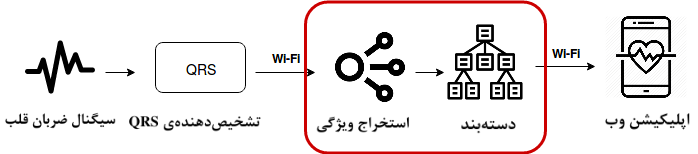
\includegraphics[width=16cm]{Figures/server.png}
\caption{بخش پردازش سمت سرور در مراحل تشخیص آریتمی}
\label{fig:server}
\end{figure}	
	

	\subsection{نحوه‌ی اجرای الگوریتم یادگیری}
		
		\subsubsection{استخراج ویژگی‌ها}
		در فرایند دسته‌بندی ضربان‌‌ها، یک مدل  \lr{SVM} با استفاده از ویژگی‌های استخراج‌شده ساخته می‌شود. همان‌طور که اشاره شد، بازه‌های \lr{RR} و میزان نوسانات آن‌ها ظرفیت بالایی در تشخیص آریتمی دارند، از طرف دیگر، در صورت استفاده از این ویژگی، داده‌های ارسالی از سمت سخت‌افزار متصل به بیمار، حجم پایینی خواهند داشت و در نتیجه تاخیر ارسال داده‌ها به سرور به حداقل خواهد رسید، که برای کاربرد بی‌درنگ ما مناسب‌تر است به همین دلیل از بازه‌های \lr{RR} برای تولید ویژگی‌ها استفاده می‌شود.
برای تولید ویژگی‌ها، با دریافت هر قله‌ی \lr{R} جدید در سرور، مقادیر زیر محاسبه می‌شوند:
\begin{itemize}
	\item \lr{Pre-RR}: این مقدار فاصله‌ی بین ضربان جاری (مربوط به قله‌ی \lr{R} دریافت‌شده و قله‌ی ضربان قبلی را نشان می‌دهد.
	\item \lr{Post-RR}: این مقدار فاصله‌ی زمانی بین قله‌ی R تازه دریافت‌شده و قله‌ی R بعدی را نشان می‌دهد.
	\item \lr{Local-RR}: میانگین ۱۰ مقدار \lr{Pre-RR} گذشته در این مقدار محاسبه می‌شود.
	\item \lr{Global-RR}: میانگین مقادیر \lr{Pre-RR}  تولیدشده در ۱۰دقیقه‌ی گذشته در این مقدار محاسبه می‌شود.
\end{itemize}

	در سرور میانگین هر یک از این چهار مقدار محاسبه شده و با رسیدن مقادیر جدید، به‌روز می‌شود. از این میانگین سپس برای نرمال‌سازی ویژگی‌هایی که تا کنون استخراج شده‌اند استفاده می‌شود، به این صورت که هر یک از این چهار ویژگی به میانگین خود تقسیم شده و چهار ویژگی دیگر را می‌سازند. در انتها ۸ ویژگی از بازه‌های \lr{RR} تولید شده و به مدل دسته‌بند تحویل داده می‌شوند.

		
		\subsubsection{ساخت مدل SVM}
پردازش‌های سمت سرور و الگوریتم \lr{SVM} به کمک زبان پایتون و فریم‌ورک \lr{Django} پیاده‌سازی شدند. زبان پایتون به دلیل پشتیبانی از کتاب‌خانه‌های متنوعی برای پیاده‌سازی انواع الگوریتم‌های یادگیری، برای استفاده در این کاربرد مناسب تشخیص داده شد. برای پیاده‌سازی الگوریتم \lr{SVM} در این زبان، از کتاب‌خانه‌ی scikit-learn استفاده کردیم. برای ساخت و آموزش یک مدل \lr{SVM}، نمونه‌ای از کلاس \lr{SVC} (از کلاس‌های عضو کتاب‌خانه‌ی \lr{scikit-learn} که برای دسته‌بندی‌های چنددسته‌ای استفاده می‌شود) ساخته شده و ویژگی‌های استخراج‌شده از داده‌های آموزش، به علاوه‌ی پارامترهای ضروری برای مدل \lr{SVM} به آن داده شدند. 

	تابع کرنل در این مدل، \lr{RBF} در نظر گرفته شده و پارامترهای مربوط به آن تعیین شده‌است. مقدار گاما در این مدل‌ها برابر با مقدار پیش‌فرض گاما در مدل‌های \lr{SVM} قرار داده شد که مساوی با $\frac{1}{number of features}$ است.
	
برای تعیین پارامتر \lr{C} در این مدل، از روش اعتبارسنجی متقابل ۱۰ لایه‌ای استفاده کردیم. در این روش، پارامتر C از مقدار ۰/۰۰۰۱ تا ۱۰۰۰۰ به صورت لگاریتمی تغییر داده شده و به ازای هر مقدار، معیارهای کارایی محاسبه شدند. اعتبارسنجی متقابل در انتها مقدار ۰/۰۰۱ رابه عنوان بهترین مقدار در این بازه برای پارامتر \lr{C} به دست آورد.
 
سپس مدل ساخته شده و آموزش داده شد. در مرحله‌ی بعد، مدل ساخته شده با کمک توابع کلاس \lr{SVC} بر روی مجموعه‌ داده‌های تست امتحان شدند، و از استراتژی رای‌دهی \lr{OVO}\LTRfootnote{One Versus One} برای این کار استفاده شد که در بخش بعد به تفصیل توضیح داده خواهد شد.
	
		\subsubsection{استراتژی رای‌دهی}
		مدل‌هایی که با استفاده از \lr{SVM} ساخته می‌شوند، تنها برای مسائل دسته‌بندی دودویی\LTRfootnote{Binary classification} قابل استفاده هستند. در این مسائل، هدف جداسازی دو کلاس از داده‌ها است. این محدودیت باعث شده است راه‌حل‌هایی ارائه شود تا بتوان از \lr{SVM} در مسائل دسته‌بندی چندکلاسی نیز استفاده کرد. دو راه‌حل اصلی و پرکاربرد برای حل این گونه مسائل، روش OVO و روش OVR\LTRfootnote{One versus Rest} است. در هر دوی این روش‌ها، مدل \lr{SVM} برای حل مسئله‌ای دودویی آموزش داده می‌شود و سپس با استراتژی‌هایی،‌ این دسته‌بندی به چند کلاس تعمیم داده می‌شود.
		 
در روش \lr{OVR} برای یک مسئله دسته‌بندی \lr{k} کلاسی،‌ به ازای هر کلاس، یک مدل \lr{SVM} آموزش داده می‌شود و تعیین می‌کند آیا یک نمونه به این کلاس تعلق دارد یا به بقیه‌ی کلاس‌ها. در این روش \lr{k} دسته‌بند دودویی داریم که بر روی نمونه‌ها اعمال می‌شوند و در انتهابه ازای هر نمونه، \lr{k} نتیجه به دست می‌آید. 
در روش \lr{OVO} تعداد $\frac{k(k-1)}{2}$ مدل \lr{SVM} دودویی متمایز آموزش داده می‌شود. این تعداد برابر با ترکیب ۲ از \lr{k} کلاس،‌ و به بیان دیگر، تعداد روش‌های انتخاب دو کلاس از بین این \lr{k} کلاس است. هر یک از این مدل‌ها یک جفت از کلاس‌های هدف را دریافت کرده و تشخیص می‌دهد یک نمونه به کدام یک از این دو کلاس تعلق دارد. در این روش به ازای هر نمونه، $C(n, 2)$ نتیجه به دست می‌آید.
در هر دوی این روش‌ها، برای تعیین نتیجه‌ی نهایی دسته‌بندی هر نمونه، یک استراتژی رای‌دهی\LTRfootnote{Voting strategy} مورد نیاز است. روش \lr{OVO} نتایج بهتری در مواردی که داده‌ها نامتعادل هستند از خود نشان داده‌است. همچنین این روش در مواردی که تعداد نمونه‌ها بسیار زیاد است،‌ زمان کمتری برای یادگیری نیاز دارد.\cite{Mondejar} به همین دلیل در این پروژه از \lr{OVO} استفاده شده‌است.

با توجه به این که در این کار‌،‌ ۴ کلاس هدف داریم، در مرحله‌ی یادگیری‌، ۶ مدل دودویی ساخته شده و بر روی هر نمونه اعمال می‌شود. در واقع در این‌جا ۶ ابرصفحه ساخته می‌شود که هرکدام، نمونه‌های  یک جفت از کلاس‌های هدف را از هم تمایز می‌دهد. در انتهای این مرحله،‌ ماتریس تابع تصمیم‌گیری\LTRfootnote{Decision function} تولید می‌شود که طول آن برابر با تعداد نمونه‌های مجموعه‌ی آموزش و عرض آن برابر با ۶ است. بر روی هر یک از این ۶ مقدار تعیین‌شده برای هر نمونه،‌لازم است یک استراتژی رای‌دهی اعمال شود. این استراتژی به صورتی که در ادامه توضیح داده خواهد شد پیاده‌سازی شده‌است.

هر یک از مقادیر تابع تصمیم‌گیری نتیجه‌ی دسته‌بندی بین یک جفت از کلاس‌ها را نشان می‌دهد. این نتیجه را مثبت یا منفی بودن مقدار نشان می‌دهد. با توجه به این مقادیر، کلاسی که بیشترین مقدار مثبت را برای یک نمونه دریافت کرده‌باشد، به عنوان کلاس برگزیده برای آن نمونه انتخاب می‌شود. 

	\subsection{نحوه‌ی پردازش داده‌های دریافت‌شده در سرور}

مراحلی که پیش‌تر توضیح داده شدند، به خصوص اعتبارسنجی متقابل، از نظر محاسبات و زمان اجرا بسیار هزینه‌بر هستند. این بخش‌ها به صورت آفلاین و بر روی کامپیوتر شخصی اجرا شدند. خروجی این مراحل یک مدل \lr{SVM} است که توانایی پیش‌بینی برچسب داده‌‌های ناشناخته و جدید را دارد. کتاب‌خانه‌ی \lr{scikit-learn} این امکان را می‌دهد که مدل \lr{SVM} حساب‌شده، در یک فایل باینری ذخیره شود. هر بار که نیاز به پیش‌بینی برچسب داده‌ی جدیدی بود، مدل \lr{SVM} را می‌توان از روی این فایل بارگیری کرده و با پاس‌دادن ویژگی‌های داده‌های جدید به آن، برچسب‌های پیش‌بینی‌شده را دریافت نمود. هزینه‌ی این کار به طرز چشم‌گیری کم‌تر از این است که مدل هر بار از روی داده‌های آموزش ساخته‌ شده و آموزش داده شود.

 پس از انتخاب بهترین پارامترها به کمک اعتبارسنجی متقابل، ساخت و ارزیابی مدل به صورت آفلاین انجام شد. این مدل بر روی فایل باینری ذخیره شده و به سرور انتقال داده شد. برای پیاده‌سازی عملیات سمت سرور، از محیط توسعه‌ی فراهم‌شده به وسیله‌ی وب‌سایت \url{pythonanywhere.com} استفاده شد. این محیط، قابلیت میزبانی اپلیکیشن‌های وب توسعه‌داده‌شده با پایتون را فراهم می‌کند.
 
 نحوه‌ی عملکرد کد سمت سرور به این صورت است که به محض دریافت داده‌‌های پیش‌پردازش‌شده‌ی جدید از سمت سخت‌افزار، این داده‌ها در پایگاه‌داده‌ی خود سرور ذخیره می‌شوند. سخت افزار برای فرستادن مقدار جدیدی به نام \lr{value} به سرور، هر بار یک درخواست \lr{HTTP} به این شکل زیر به سرور می‌فرستد:
\lr{GET /store/\{value\}}
 
کاربر برای دیدن نتایج پردازش‌ها، کافی است \lr{URL} دامنه را در مرورگر خود وارد کند، و در واقع یک درخواست \lr{HTTP GET} به مسیر / بزند. این درخواست در سرور به این صورت مدیریت می‌شود که ابتدا مدل \lr{SVM} از روی فایل بارگیری شده، سپس آخرین داده‌‌های پیش‌پردازش‌شده که تا کنون در پایگاه‌داده ذخیره شده‌اند، به مدل داده می‌شوند تا کلاس آن‌ها پیش‌بینی شود. سپس نتیجه در مرورگر به کاربر نشان داده خواهد شد. 
 
برای آسان‌تر بودن استفاده برای کاربر، صفحه‌ی وب طراحی شده به صورت خودکار و هر یک ثانیه یک بار بارگیری می‌شود. با فرض این که سخت‌افزار به طور مرتب قله‌های \lr{R} تشخیص‌داده‌شده را برای سرور بفرستد، در هر ثانیه یک درخواست \lr{GET} به مسیر / زده شده و کلاس‌های داده‌های جدید به وسیله‌ی مدل، پیش‌بینی و بر روی صفحه‌ی وب نمایش داده می‌شوند. با توجه به این که به طور تقریبی در هر ثانیه یک ضربان قلب تولید می‌شود، چنین کاربردی به صورت بی‌درنگ و با تاخیری اندک نتایج دسته‌بندی هر ضربان را به کاربر نشان می‌دهد. نمونه‌ای از خروجی نشان‌داده‌شده به کاربر در مرورگر، در شکل \ref{fig:website} قابل مشاهده است.

\begin{figure}[!htb]
\centering
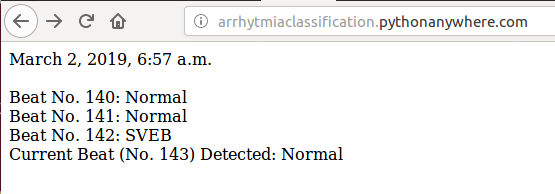
\includegraphics[width=15cm]{Figures/website.png}
\caption{خروجی نشان‌داده‌شده در مرورگر}
\label{fig:website}
\end{figure}	

	\subsection{داده‌های مورد بررسی در الگوریتم یادگیری}
	به منظور استانداردسازی الگوریتم‌های گوناگون تشخیص آریتمی، لازم است ارزیابی این الگوریتم‌ها بر روی مجموعه داده‌های استاندارد و مشترکی صورت بگیرد تا در مقایسه‌ی نتایج حاصل از آن‌ها با دقت کافی حاصل شود. برای این منظور، تعدادی پایگاه‌داده از نمونه‌های ضربان قلب توسط موسسه‌های گوناگون گردآوری شده است. انجمن پیشبرد ابزار دقیق پزشکی\LTRfootnote{Association for the Advancement of Medical Instrumentation (AAMI) } که به اختصار \lr{AAMI} نامیده می‌شود، تعدادی از این پایگاه‌داده‌ها را به عنوان منابع استاندارد داده برای ارزیابی الگوریتم‌های تشخیص آریتمی معرفی کرده و هم‌چنین قراردادهایی برای اجرای عملیات ارزیابی الگوریتم‌ها در آن تعیین کرده‌است، تا کاملا از تکرارپذیری و قابل‌مقایسه‌بودن نتایج آزمایش‌های متفاوت اطمینان حاصل شود. در این استاندارد، استفاده از ۵ پایگاه‌داده‌ی زیر توصیه شده است:
\begin{itemize}
	\item پایگاه‌داده‌ی \lr{MIT-BIH}\LTRfootnote{Massachusetts Institute of Technology - Beth Israel Hospital} شامل ۴۸ نوار قلب ۳۰ دقیقه‌ای
	\item پایگاه‌داده‌ی \lr{EDB}: شامل ۹۰ نوار قلب ۲ ساعته
	\item پایگاه‌داده‌ی \lr{AHA} شامل ۸۰ نوار قلب ۳۵ دقیقه‌ای
	\item پایگاه‌داده‌ی \lr{CU} شامل ۳۵ نوار قلب ۸ دقیقه‌ای
	\item پایگاه‌داده‌ی \lr{NST} شامل ۱۲ نوار قلب ۳۰ دقیقه‌ای
\end{itemize}	 
از بین این موارد، \lr{MIT-BIT} که در این پروژه از آن استفاده کرده‌ایم، اولین پایگاه‌داده‌ی به‌وجودآمده برای این منظور، و پرکاربردترین مجموعه داده برای دسته‌بندی و ارزیابی الگوریتم‌های تشخیص آریتمی است.\cite{ECGSurvey} در ادامه این پایگاه‌داده را دقیق‌تر بررسی خواهیم کرد. 


		\subsubsection{پایگاه‌داده‌ی MIT-BIH}
		برچسب‌گذاری‌های ضربان‌ها در \lr{MIT-BIH} در طی سال‌ها به طور دائم بهبود داده شده‌اند. به دلیل گستردگی داده‌ها و وجود انواع ضربان‌قلب در این نمونه‌‌ها، بیشترین پژوهش‌ها بر روی این پایگاه‌داده‌ انجام گرفته‌اند.\cite{ECGSurvey} 
در \lr{MIT-BIH} تمامی ضربان‌ها به وسیله‌ی یک الگوریتم تشخیص \lr{QRS} از یک‌دیگر متمایز شده‌اند و به هر تک‌ضربان قلب، برچسبی اختصاص داده شده است که نوع آن ضربان  را تعیین می‌کند. این برچسب‌ها در برای پیاده‌سازی و ارزیابی الگوریتم‌های تشخیص آریتمی ضروری هستند. نحوه‌ی انجام این برچسب‌گذاری نیز در استاندارد \lr{AAMI} تعیین شده‌است.

با وجود تنوع انواع ضربان‌قلب‌های دارای آریتمی، ترجیح \lr{AAMI} بر استفاده از ۱۵ کلاس از بین این انواع است. این ۱۵ کلاس، خود به ۵ کلاس کلی‌تر طبقه‌بندی شده‌اند: 
\begin{enumerate}
	\item ضربان‌های عادی\LTRfootnote{Normal} \lr{(N)}
	\item ضربان‌های نابه‌جای فوق بطنی\LTRfootnote{Supraventricular ectopic beats} \lr{(SVEB)}
	\item ضربان‌های نابه‌جای بطنی\LTRfootnote{Ventricular ectopic beats} \lr{(VEB)}
	\item ضربان‌‌های ادغام‌شده\LTRfootnote{Fusion beats} \lr{(F)}
	\item ضربان‌های ناشناخته\LTRfootnote{Unknown beats} \lr{(Q)}
\end{enumerate}

این پایگاه‌داده‌ شامل ۴۸ نوارقلب با نرخ نمونه‌برداری ۳۶۰ هرتز است. این نوارقلب‌ها از ۴۷ بیمار گرفته شده‌اند و هر کدام مدت‌زمانی برابر با ۳۰ دقیقه دارد. هر نوارقلب، شامل نمونه‌های دو لید مجزا است. در بیشتر نوارقلب‌ها، لید اصلی که لید \lr{A} نام دارد، نمونه‌ی تغییریافته‌ای از لید \lr{II} است که از الکترودهای قرارگرفته بر روی سینه به دست می‌آید. لید دوم که لید \lr{B} نام دارد، در بیشتر نوارقلب‌ها لید \lr{V1} و در دیگران \lr{V2}, \lr{V4} و یا \lr{V5} است. عموما برای تشخیص آریتمی از لید اول \lr{(A)} استفاده می‌شود، چرا که در این لید، موج \lr{QRS} واضح‌تر است.\cite{ECGSurvey}

پایگاه‌داده‌های موجود از نظر تعداد ضربان‌های متعلق به هر کلاس آریتمی، شدیدا نامتعادل\LTRfootnote{Imbalanced} هستند. \lr{MIT-BIH} تنها پایگاه‌داده‌ای است که هر ۵ کلاس آریتمی ذکرشده را پوشش می‌دهد. اما در این پایگاه‌داده نیز، حدود ۹۰ درصد ضربان‌ها در کلاس \lr{N} جای می‌گیرند و از ۱۰ درصد باقی‌مانده، حدود ۳٪، ۶٪ و ۱٪ به ترتیب متعلق به کلاس‌های \lr{SVEB}، \lr{VEB} و \lr{F} هستند، و درصد ضربان‌های کلاس \lr{Q} پایین‌تر از ۱ درصد است.\cite{Mondejar} به همین دلیل، لازم است در الگوریتم‌های دسته‌بندی و روش‌های ارزیابی آن‌ها، نامتعادل‌بودن پایگاه‌داده مد نظر قرارگیرد.

		\subsubsection{نحوه‌ی تقسیم داده‌ها به دو مجموعه‌ی آموزش و تست}
		دو الگوی اصلی برای ارزیابی روش‌های اتوماتیک تشخیص آریتمی استفاده می‌شود: الگوی درون‌بیماری\LTRfootnote{Intra-patient paradigm} و الگوی بین‌بیماری\LTRfootnote{Inter-patient paradigm}. در الگوی اول، هیچ‌گونه محدودیتی در تقسیم پایگاه‌داده به دو بخش آموزش و تست وجود ندارد و هر یک از ضربان‌قلب‌های موجود را می‌توان صرف نظر از این که متعلق به کدام بیمار است، در هر یک از این دو مجموعه جای داد. این نوع تقسیم بندی، یک نقص اساسی دراین روش تقسیم‌بندی را موجب می‌شود. از آن جا که در حین یادگیری، امکان دارد مدل تولید شده بتواند الگوهای موجود در ضربان‌های یک بیمار خاص را نیز تشخیص داده و یادبگیرد، نتایج ارزیابی به‌دست‌آمده از الگوریتمی که با الگوی درون‌بیماری کار می‌کند، نمی‌تواند کاملا قابل اعتماد باشد. چرا که به طور مطلوب، یک الگوریتم دسته‌بندی آریتمی باید بتواند برای هر بیماری، با دقتی معین عمل کند، حتی اگر سیستم از پیش اطلاعی در مورد آن بیمار نداشته‌باشد. 
در راستای ارزیابی واقع‌گرایانه‌تر، الگوی بین‌بیماری توسط \lr{Chazal} و همکاران معرفی شد.\cite{deChazal2004} در این الگو تقسیم‌بندی پایگاه‌داده به دو مجموعه‌ی یادگیری و ارزیابی، طوری صورت می‌گیرد که هیچ ضربانی از یک بیمار خاص در هر دو مجموعه به طور هم‌زمان حاضر نباشد. نحوه‌ی تقسیم‌بندی داده‌ها در استاندارد ارائه‌شده به صورت زیر می‌باشد:
\begin{itemize}
	\item مجموعه‌داده‌ی اول \lr{(DS1)} شامل نوارقلب‌های 101, 106, 108, 109, 112, 114, 115, 116, 118,
119, 122, 124, 201, 203, 205, 207, 208, 209, 215, 220, 223 و
230
	\item مجموعه‌داده‌ی دوم \lr{(DS2)} شامل نوارقلب‌های 100, 103, 105, 11, 113, 117, 121, 123,
200, 202, 210, 212, 213, 214, 219, 221, 222, 228, 231, 232, 233
و 234
\end{itemize}
 همان‌طور که اشاره شد، ارزیابی مدل‌ها با استفاده از این الگو، نتایج قابل‌اعتمادتری ارایه می‌کنند. این روش تقسیم‌بندی پس از معرفی، به طور گسترده‌ای در کارهایی که با الگوی بین‌بیماری کار می‌کنند به کار رفته‌است. در این پروژه نیز از این الگو برای ارزیابی بهره گرفته شده‌است. 



	\subsection{ارزیابی نتایج حاصل از یادگیری}
	معیارهای دقت، صحت، صحت کلی و حساسیت (که در بخش \ref{sec:performance} توضیح داده شدند) توسط \lr{AAMI} برای ارزیابی روش‌های مختلف پیشنهاد شده‌اند. 
به دلیل نامتعادل بودن پایگاه‌داده‌های موجود، صحت کلی نمی‌تواند معیار مناسبی برای سنجش باشد. در\lr{MIT-BIH} به دلیل پر تعداد بودن ضربان‌های متعلق به کلاس \lr{N} که حدود ۹۰ درصد داده‌ها را به خود اختصاص داده‌اند،‌ این کلاس در محاسبه‌ی صحت کلی بر دیگر کلاس‌ها شدیدا غالب می‌شود. به همین دلیل، این معیار به طور معمول برای مقایسه‌ی الگوریتم‌ها مورد استفاده قرار نمی‌گیرد.

\subsubsection{معیارهای کارایی}
\label{subsec:perf}
علاوه بر چهار معیار ذکرشده، معیارهای دیگری توسط \lr{AAMI} به عنوان معیارهای استاندارد معرفی شده‌اند. این معیارها از ماتریس درهم‌ریختگی استخراج می‌شوند و طبق  استاندارد‌، استثنائاتی در محاسبه‌ی آن‌ها در نظر گرفته می‌شود. برای مثال، در صورتی که الگوریتم دسته‌بندی، ضربانی از کلاس \lr{F} را به اشتباه متعلق به کلاس \lr{VEB} تشخیص دهد، در میزان موفقیت یا خطای الگوریتم تاثیری نخواهد داشت. 
همان‌طور که ذکر شد، صحت کلی نمی‌تواند میزان موفقیت یک الگوریتم در دسته‌بندی ضربان‌ها را به خوبی نشان دهد. برای غلبه بر این مشکل، یک مقدار جدید به نام اندیس \lr{j$\kappa$} توسط \lr{Mar} و همکاران معرفی شده است.\cite{Mar2011} این مقدار مجموع وزن‌داری از اندیس \lr{j} و کاپای کوهن ($\kappa$) است.

اندیس \lr{j} (رابطه‌ی \ref{eq:jindex}) به پیروی از استاندارد \lr{AAMI}، دقت تمایزدهی مهم‌ترین کلاس‌های آریتمی، یعنی \lr{VEB} و \lr{SVEB} را اندازه‌گیری می‌کند.\cite{Mondejar}
\begin{equation}
	j\:index = Se_{SVEB} + Se_{VEB} + P^+_{SVEB} + P^+_{VEB}
	\label{eq:jindex}
\end{equation}

کاپای کوهن مقداری قراردادی برای ارزیابی نتایج موجود در ماتریس درهم‌ریختگی است. کاپا به عنوان معیاری مقاوم‌تر به نسبت صحت کلی برای پایگاه‌داده‌های نامتعادل گزارش شده‌است. در این رابطه، $P_o$ که احتمال مشاهده‌شده\LTRfootnote{Observed probability} نام دارد، مساوی با صحت کلی است،‌ و مقداری دیگر به نام $P_e$ نیز تعریف می‌شود. در محاسبه‌ی این مقدار، تعداد نمونه‌های موجود در هر کلاس لحاظ شده‌است و به این دلیل برای مقایسه‌ی عملکرد در پایگاه‌داده‌های نامتعادل مناسب است. 

\begin{equation}
\begin{split}
	& \kappa = \frac{P_o - P_e}{1 - P_e} \\
	& P_o = \frac{Nn+Ss+Vv+Ff}{\Sigma} \\
	& P_e = \frac{\Sigma N \Sigma n + \Sigma S \Sigma s + \Sigma V \Sigma v + \Sigma F \Sigma f}{\Sigma^2}
\end{split}
\end{equation}

اندیس \lr{j$\kappa$} به صورت رابطه‌ی \ref{eq:jkindex} محاسبه می‌شود. وجود $\kappa$ باعث می‌شود نرخ دسته‌بندی نادرست\LTRfootnote{Misclassification rate} و همین‌طور تعداد نمونه‌های موجود در هر کلاس در محاسبه‌ی این معیار مد نظر قرارداده شود. به طور هم‌زمان، میزان تشخیص \lr{VEB} و \lr{SVEB} نیز که در محاسبه‌ی اندیس \lr{j} لحاظ شده‌اند،‌ در این مقدار دخالت دارند. تمامی این مقادیر،‌ اندیس \lr{j$\kappa$} را به معیاری مناسب برای مقایسه‌ی الگوریتم‌های دسته‌بندی آریتمی تبدیل کرده است.  
\begin{equation}
	j\kappa\:index = w_1\kappa + w_2(j\:index)
\label{eq:jkindex}
\end{equation}



%------------------------ End chapter 3 -------------
